\section{Output}
\label{sec:output}

After a log file is consumbed by PET, its output should have to be usable for
many different aspects. On early basis or when big differences are excepected, a
sparse annotated graphical output might be the best way of displaying where most
power is consumbed, but as the project evolves and mose subtile changes are
evaluated, a textual output will be easier to compare. PET supports three
different output options:

\begin{description}
    \item[plain]\hfill\\
        The example in \autoref{lst:pet_output_plain} shows the simple
        \emph{plain}-format, which is a simple output format intended for
        use as input for further processing.
    \item[table]\hfill\\
        The table format, with an example shown in \autoref{lst:pet_output_table},
        shows a terminal-printable output which is easier to understand by
        humans, and is intended for further study of the numbers. This might
        come in handy as the last format, GNUPlot-graph, might be hard to
        read when you are out after very specific information.
    \item[graph]\hfill\\
        This last format is the default, and will try to give an overview of
        the entire program in a easy digestible format. An example of such
        a graph is printed in \autoref{fig:annot}.
\end{description}

\subsection{Units}

The output format is understood as timeslots in which the architecture has a
certain current drain, which should be multiplied with applied voltage to get
numbers on consumed energy, heat generation and so on. The numbers are given as
milliamperes, which is equal to milliwatt if voltage is $1~V$. PET displays its
output as $mA$ as it was easier to find current drain rather than wattage using
our test bench. As described in \autoref{sec:energymeasure}, current can be
found measuring the voltage drop of the core supply rail over a shunt resistor,
finding wattage meant that we also had to monitor the exact voltage drop over
the entire circuit, correlate these numbers in time, and multiply them together.

When power is estimated for a new architecture, the resistance of the circuit is
hard to guess, and voltage might also be an unknown factor. Given Ohms law in
\autoref{eq:ohm} and the definition of electric power in \autoref{eq:power}

\begin{equation}
I=\frac{U}{R}
\label{eq:ohm}
\end{equation}

\begin{equation}
P=U \cdot I
\label{eq:power}
\end{equation}

it can be found that power equals current squared times resistance

\[U=R \cdot I\]
\[P=(R \cdot I) \cdot I\]
\begin{equation}
P=I^2 \cdot R
\label{eq:currentsquared}
\end{equation}
and that power equals voltage squared divided by resistance
\[P=U \cdot \frac{U}{R}\]
\begin{equation}
P=\frac{U^2}{R}
\label{eq:voltagesquared}
\end{equation}

Thus, estimating only the current drain means that the power at each point will
be known without knowing resistance or voltage, further, energy comsumption can
not be estimated unless the new architecture is mostly equal in voltage and
resitance to a chip where these numbers are available. Even the current drain
might not be representable at all; if resitance or voltage is far away from the
levels found in the reference chip, the final numbers will be far off.

From \autoref{eq:currentsquared} and \autoref{eq:voltagesquared} it is easy to
see that voltage and current is very imporant for power and then also enery. The
current is, from \autoref{eq:ohm}, dependent on resistance as well as voltage.
With this in mind, and knowing that power in a complex environment is a delicate
matter, the most important application for a simple tool as PET this early in
the design phase is to point in the right direction. PET will never give
accurate power estimations for new chips, but will guide you on the way to
figyre out if a new feature or architectural fix will render the final
architecture more energy efficient.


\subsection{Examples of Output Data}

Example of the \texttt{plain} output format can be seen in
\autoref{lst:pet_output_plain}. The left column is the bucket number, while the
right column is instant current draw from the modelled architecture.

\begin{lstlisting}[float=hbt,label={lst:pet_output_plain},caption={PET Plain Output with annotations}]
0 120 memcpy
1 113 start
2 150 main
3 123 main
4 133 fun1
5 117 main
\end{lstlisting}

When reading the output directly from console, a more descriptive output format
is the \texttt{table} format. An example using this option is rendered in
\autoref{lst:pet_output_table}.

\begin{lstlisting}[float=hbt,label={lst:pet_output_table},caption={PET Table Output with annotations}]
/----------------------------------------\
|   Bucket   |  milliAmps |    Symbol    |
|------------|------------|--------------|
|          0 | 120.000000 |    memcpy    |
|          1 | 113.000000 |    start     |
|          2 | 150.000000 |    main      |
|          3 | 123.000000 |    main      |
|          4 | 133.000000 |    fun1      |
|          5 | 117.000000 |    main      |
\----------------------------------------/
\end{lstlisting}

Visualization is often a good thing when inspecting old or trying to understand
new problems. As it is hard to get a good overview from huge text log files, PET
provides, as stated in \autoref{subsec:annot}. In effect, it is formatting
temporary output files and calling GNUPlot do do the hard work.

\begin{figure}[htb]
    \centering
    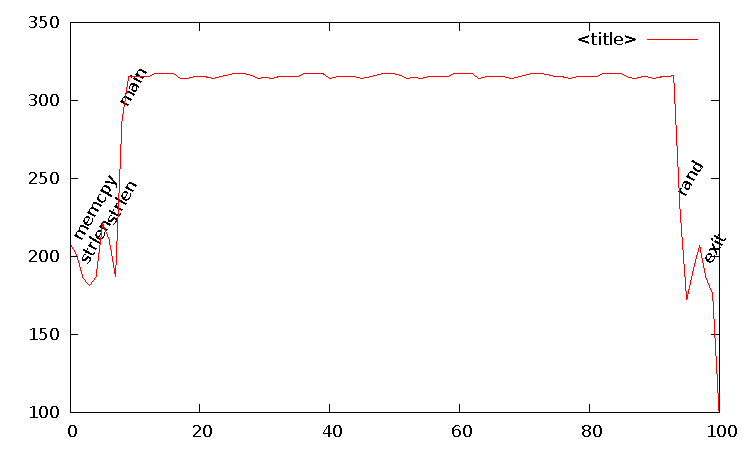
\includegraphics[width=0.9\textwidth]{figs/annot.pdf}
    \caption{PET Graphical Output with annotations}
    \label{fig:annot}
\end{figure}

